\newpage
\subsection{Box-Line Reduction}
Die Technik \textit{Box-Line-Reduction} ist verwandt mit der Technik \textit{Pointing Pair / Triple}. Hier wird das Sudoku zeilen- und spaltenweise betrachtet. Ist das Vorkommen einer Zahl in den Kandidatenlisten auf einen Block beschränkt, dann kann jedes weitere Vorkommen der Zahl aus den Kandidatenlisten der Zellen des selben Blocks gestrichen werden, die nicht in der Zeile oder Spalte liegen. Die Begründung dafür ist ähnlich der Begründung bei \textit{Pointing Pair / Triple}. Da die Zahlen 1 bis 9 jeweils genau einmal in der Zeile oder Spalte vorkommen müssen und dieses Vorkommen auf einen Block beschränkt ist, ist klar, dass die Zahl letztendlich in diesem Block vorkommt und zwar in der gefundenen Zeile oder Spalte. Die Zahl kann aber nicht zweimal in dem Block vorkommen, daher kann sie aus den Kandidatenlisten des Blocks gelöscht werden, deren Zellen sich nicht in der Reihe oder Spalte befinden.

\begin{figure}[h]
\begin{center}
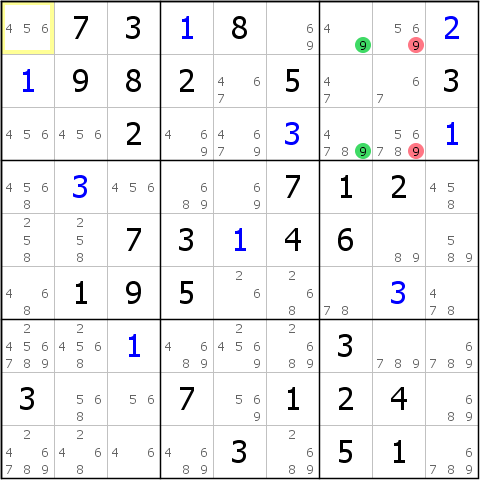
\includegraphics{./img/box_line_reduction.png}
\caption{Box-Line Reduction}
\end{center}
\end{figure}

Wir betrachten Spalte 6 in \textbf{Abbildung 3.5}. Hier sieht man, dass das Vorkommen der Zahl 4 in dieser Spalte auf Block 2, den oberen Block, beschränkt ist. Anhand dieser Spalte sieht man also, dass die Zahl 4 entweder in z2s6 oder in z3s6 steht, also in jedem Fall in Block 2. Daher kann die Zahl 4 aus den Kandidatenlisten der anderen Zellen in Block 2 gestrichen werden.
